\documentclass[stu,12pt,floatsintext,a4paper]{apa7}
% Options used in this document (general note - for each of these, if you want to use the other options, swap it out in that spot in the square brackets):
% - stu: this sets the `document mode' as the "student paper" version. Other options are jou (journal), man (manuscript, for journal submission), and doc (a plain document)
% --- The student setting includes things like 'duedate', 'course', and 'professor' on the title page. If these aren't wanted/needed, use the 'man' setting. It also defaults to including the tables and figures at the end of the document. This can be changed by including the 'floatsintext' option, as I have for you. If the instructor wants those at the end, remove that from the square brackets.
% --- The manuscript setting is roughly what you would use to submit to a journal, so uses 'date' instead of 'duedate', and doesn't include the 'course' or 'professor' info. As with 'stu', it defaults to putting the tables and figures at the end rather than in text. The same option will bump those images in text.
% --- Journal ('jou') outputs something similar to a common journal format - double columned text and figurs in place. This can be fun, especially if you are sumbitting this as a writing sample in applications.
% --- Document ('doc') outputs single columned, single spaced text with figures in place. Another option for producing a more polished looking document as a writing sample.
% - 12pt: sets the font size to 12pt. Other options are 10pt or 11pt
% - floatsintext: makes it so tables and figures will appear in text rather than at the end. Unforunately, not having this option set breaks the whole document, and I haven't been able to figure out why. IT's GREAT WHEN THINGS WORK LIKE THEY'RE SUPPOSED TO.
\usepackage{booktabs}
\usepackage{multirow}
\usepackage[ngerman,american]{babel}
%\usepackage[american]{babel} %english ony
\usepackage{csquotes} 
\usepackage[style=apa,sortcites=true,sorting=nyt,backend=biber]{biblatex}
% biblatex: loads the package that will handle the bibliographic info.
% - style=apa: sets the reference format to use apa (albeit the 6th edition)
%\DeclareLanguageMapping{american}{american-apa} %english ony
\DeclareLanguageMapping{ngerman}{ngerman-apa}
% Koschutnig: Hier wird Ihre Bibliographie definiert!
\addbibresource{bibliography.bib} 
\usepackage[T1]{fontenc} 
\usepackage{mathptmx}

% Title page stuff _____________________
% =================== USER EDITABLE METADATA ===================
% Students: Edit ONLY the commands below. Do NOT change other
% parts of this file unless you know what you're doing.
% - Replace the values inside the braces for these commands.
% - Keep the command names intact so the template keeps working.
% ----------------------------------------------------------------
\newcommand{\thesisTitle}{\enquote{Ein Leben on Word}: Warum es Sinn macht Latex zu verwenden}
\newcommand{\thesisSemester}{WS2018/19}
\newcommand{\thesisSupervisor}{Herr Assoz. Univ. – Prof. Mag. Dr. Harry Hirsch}
\newcommand{\thesisAuthor}{Susi Sorglos}
\newcommand{\department}{Biologische Psychologie}
\newcommand{\thesisDate}{04.02.2019}
\newcommand{\shortTitle}{Word is not good}
% ----------------------------------------------------------------
% End of USER EDITABLE METADATA
% ==============================================================

\title{Bachelorarbeit: \thesisTitle} % The big, long version of the title for the title page
\shorttitle{\shortTitle} % The short title for the header (defined in preamble)
\author{\thesisAuthor}
\duedate{\thesisSemester}
% \date{January 17, 2024} The student version doesn't use the \date command, for whatever reason
\affiliation{Institut für Psychologie, Karl-Franzens-Universität Graz \\ \vspace{1cm} \includegraphics[width=3cm]{figures/uni-graz-logo.pdf}}
% \course removed: students don't need to edit course in this template
\professor{\thesisSupervisor} 

\begin{document}

% Custom Title Page matching the screenshot
\begin{titlepage}
    \thispagestyle{empty} % No header on title page
    
    \noindent
    \begin{minipage}[c]{0.2\textwidth}
        \mbox{} % Empty box for spacing
    \end{minipage}%
    \begin{minipage}[c]{0.6\textwidth}
        \centering
        {\fontsize{32}{40}\selectfont \textbf{Bachelorarbeit}\par}
    \end{minipage}%
    \begin{minipage}[c]{0.2\textwidth}
        \raggedleft
        \includegraphics[width=0.8\linewidth]{figures/uni-graz-logo.pdf}
    \end{minipage}

    \vspace{1cm}

    \centering
    {\normalsize Im Rahmen der Lehrveranstaltung\par}
    \vspace{0.3cm}
    {\normalsize Seminar Forschungsmethodik in einem Grundlagen- oder Anwendungsfach: \department\par}
    \vspace{0.3cm}
    {\normalsize \thesisSemester\par}

    \vspace{1.5cm}

    {\Large \textbf{\thesisTitle}\par}

    \vspace{1.5cm}

    {\Large \thesisAuthor\par}

   \vspace{1.5cm}

    {\normalsize Eingereicht am \thesisDate \par}
    \vspace{0.3cm}
    {\normalsize Institut für Psychologie \par}
    \vspace{0.3cm}
    {\normalsize der Karl-Franzens-Universität Graz \par}
    \vspace{0.3cm}
    {\normalsize Bei \thesisSupervisor \par}
\end{titlepage}
\newpage

% Acknowledgment section, now manually inserted before the abstract
\section*{Acknowledgments}
I would like to thank my colleagues, mentors, and family for their support during the course of this study.
\newpage
% The abstract section, which now appears after Acknowledgments
\section*{Abstract}{This is the abstract for this paper, wherein the main points of the introduction, method, results, and discussion are quickly talked about. Probably in more than one sentence, though. Dare I guess, more than two? There is a page break before starting the Introduction.}
\newpage

Begin your paper with the introduction. The active voice, rather than the passive voice (i.e., the zombie voice), should be used in your writing.

Since the Introduction is where references in papers first show up, let us incorporate some now. Referencing  is done  for us with the right command, like  \textcite{Sample2024}. But maybe you want to just include it all at as a: \textbf{parenthetical}? \parencite{Fink2021, Contributor2023, Sample2024}. 

\section{Method}


\subsection{Participants}

Talk about the people who participated in your study. How many students, sourced from where, reimbursed how, ethics assured by what?

\begin{table}[ht]
\centering
\caption*{\textbf{Table 1} \\ \textit{Demographics of Participants Included in the Study}}
\begin{tabular}{lcccccc}
\toprule
\multirow{2}{*}{Participant ID} & \multirow{2}{*}{Age} & \multirow{2}{*}{Sex} & \multicolumn{2}{c}{ADS Score} \\
\cline{4-5}
 & & & Male & Female \\
\midrule
P001 & 29 & Male & 15 & - \\
P002 & 34 & Female & - & 12 \\
P003 & 41 & Male & 18 & - \\
P004 & 27 & Female & - & 14 \\
P005 & 38 & Male & 16 & - \\
P006 & 31 & Female & - & 13 \\
P007 & 45 & Male & 20 & - \\
P008 & 33 & Female & - & 17 \\
\bottomrule
\end{tabular}
\label{tab:demographics}
\end{table}

\subsection{Materials}


Sometimes it can be helpful to include the stimuli used in the experiment. For example, here is an example table (Table \ref{tab:table_words}) of words that were used in this hypothetical experiment. If you make use of the label command, \LaTeX{} will handle numbering things for you.

\begin{table}
    \caption{Sample words from this hypothetical experiment.}
    \centering
    \begin{tabular}{cc} %The c's here indicate the columns will be centered
        \hline 
         First word & Second word \\
         \hline
         Yeet & Yoink \\
         Hot & Lit \\
         \hline
    \end{tabular}
    \label{tab:table_words}
\end{table}

\section{Results}

Some instructors will want things broken down with the subheadings (e.g., `Descriptive Statistics') I have included, some will light your paper on fire if you \textit{do} include these. Always check with the assignment/rubric for what is wanted. Also, don't check my math on these, I am making all of the numbers up as we go, so it's almost certainly not going to hang together correctly.

I'll add this tip in here: since \LaTeX{} uses the percent symbol as the signal to comment out/hide what's typed after it in that line, what do you do if you need that symbol? You add what's called the `escape character' in front of it - the backslash. So, it would look like this: 21\%. Boom, you've got a percent symbol in text. Same goes for an ampersand: \&.

\subsection{Descriptive Statistics}

In this portion, you describe the data obtained. This includes things like the counts, means, and standard deviations. This may be omitted or rolled into the rest of the statistical discussion, so as always, check with what is being asked of you. If it is wanted as a separate section, check to see if it would be acceptable to include things as a table, a figure, or if it would be better to write it out in text. We are going to use a figure.

\begin{figure}
    \centering
    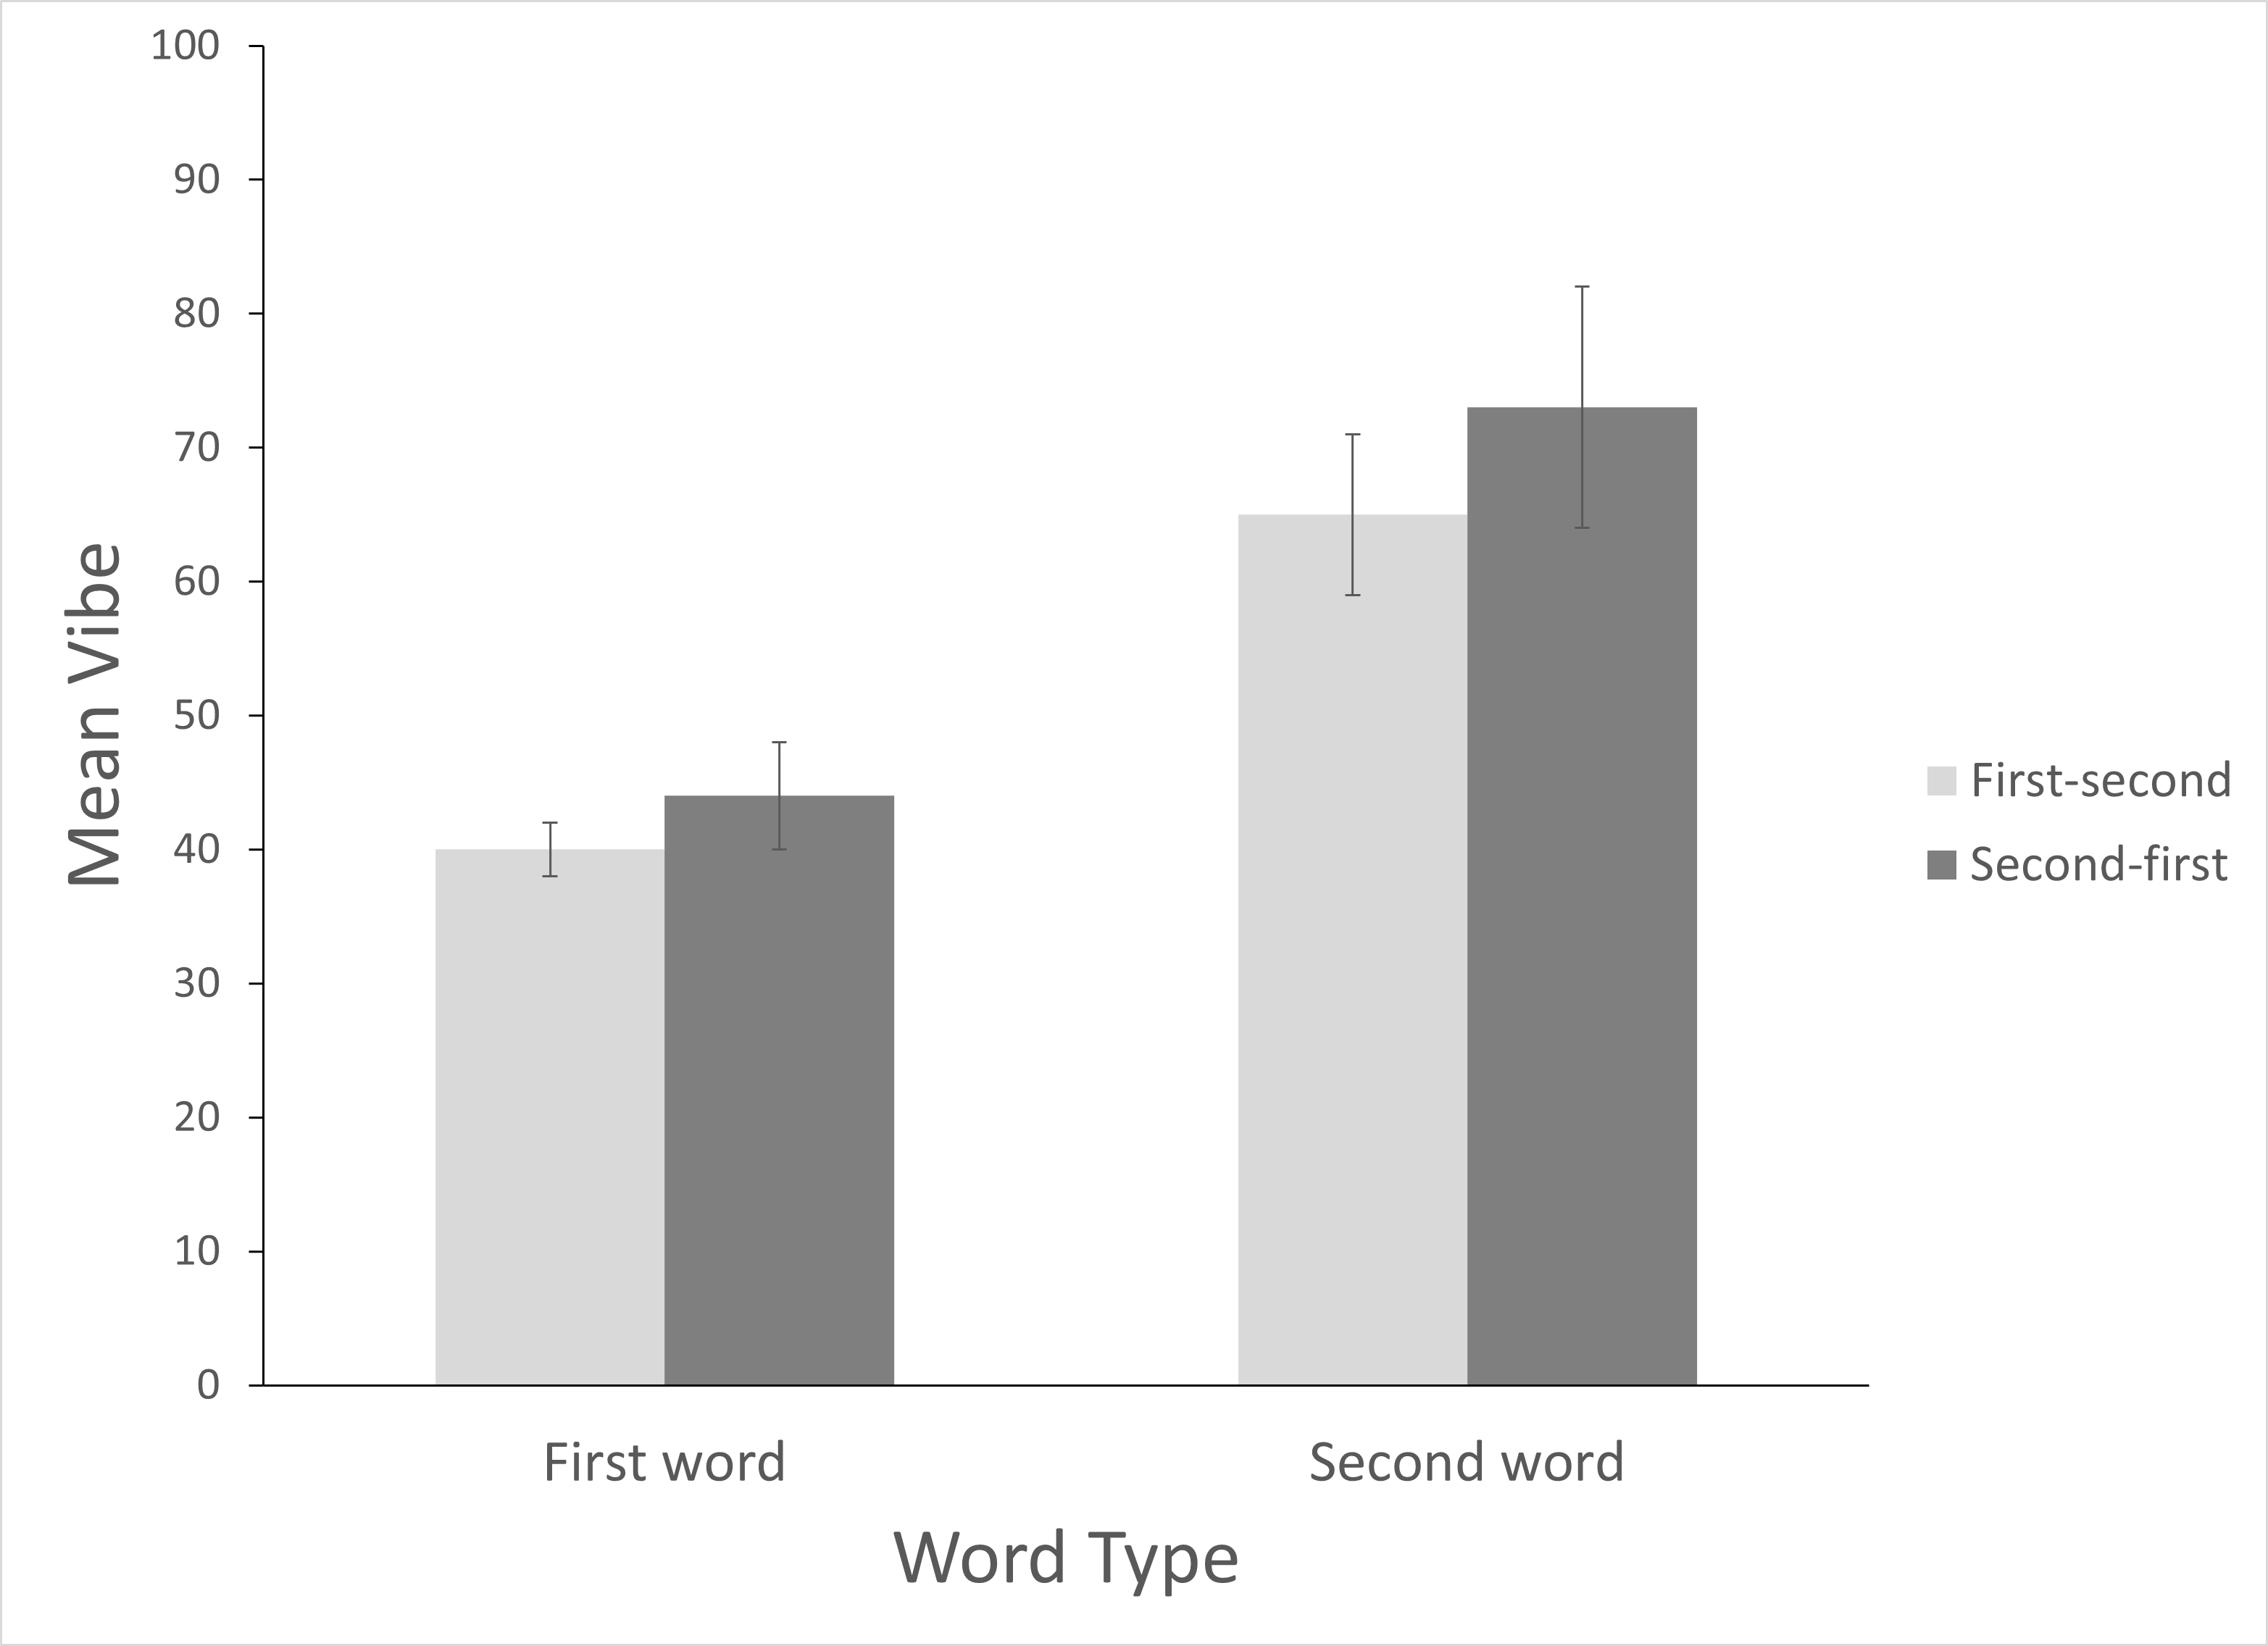
\includegraphics[width=0.75\linewidth]{figures/sampleFig.png} % This is setting the figure to be .75x the width of the line. This can go all the way from 0.1 to 1 (and beyond, but then you're outside the page).
    \caption{The mean vibes for each word type and counterbalanced condition order. Error bars represent one standard error of the mean.}
    \label{fig:OverallEffect}
\end{figure}

Figure~\ref{fig:OverallEffect} shows the means and standard errors for the four experimental groups. As shown, the mean vibes for the second word ($M = $ 69, $SE = $ 7.5) were greater than the first word ($M = $ 42, $SE = $ 3), but roughly equivalent between presentation order conditions. Another fun little \LaTeX{} thing here: your instructor may explicitly want you to use $M$, but one of \LaTeX{}'s strengths is the easy of ``math mode'' (i.e., everything enclosed by the dollar signs). %In math mode, you can easily throw in Greek characters. So you \textit{could} instead present the descriptive statistics as ($\mu = $ 42). Oooh. Shiny. Although that seems to make Overleaf work extra hard, so I keep seeing a message encouraging upgrading to a paid plan, so I've commented this part out.

\subsection{Inferential Statistics}

This is where you start to do the actual statistical analysis. We generally tell students not to \textit{interpret} what the results mean until the discussion, but pay attention when reading journal articles - realistically a bit of interpretation does tend to happen at this point in published works.

A benefit of using \LaTeX{} is the ease in adding in macros to simplify your life. A common place I rolled these out in my dissertation were to make the formatting of all the analyses correct without a lot of work. I will include a couple example macros in the editor-side now, then use them in text. But, \textbf{another pro tip:} if you are going to deploy these macros, I would get in the habit of putting them up in the preamble so they are easier to find. Also, if you really get on board the \LaTeX{} train (which you should), you can recycle the preamble between projects, so those macros will also come along for the ride.

% A macro will have this format \newcommand{macroNameYoullUseToCallIt}[Number of inputs]{What the macro does} 
% The #s indicate where information will be slotted in when the macro is used
% The dollar signs indicate "math mode" is being used. It's mandatory for some functionality (like super/subscripts) or accessing the Greek alphabet used in statistical reporting.
% These macros are including the amount of info we expected from students when I was TAing labs. You can fill them out further if more info is required - just make sure you update the number in the square brackets!
\newcommand{\ttestSig}[2]{$t$(#1) = #2, $p < .05$}
\newcommand{\ttestInsig}[2]{$t$(#1) = #2, $p > .05$}
\newcommand{\anovaSig}[3]{$F$(#1,#2) = #3, $p < .05$}
\newcommand{\anovaInsig}[3]{$F$(#1,#2) = #3, $p > .05$}

Using the hypothetical experiment we have set up, let's say there was a significant interaction found between the word conditions (first versus second) and exposure order (first-second versus second-first), \anovaSig{11}{111}{4.20}. Pairwise comparisons indicate that this was driven by the words themselves, as there was a significant difference between the words, \ttestSig{111}{3.21}, but not for the exposure order, \ttestInsig{111}{.42}.

\section{Discussion}

As mentioned at the close of the Introduction, the Discussion starts out specific before building out to the broader picture. This will typically mean that the discussion starts with a reiteration of the Results, with more emphasis on interpretation. What differences were (or were not) found? Does this support your predictions, or have you failed to reject the null hypothesis? Statements of that nature.

With that done, you can work to tie your findings into the existing literature. Perhaps this result supports the work of \textcite{Contributor2023} but contradicts others \parencite[e.g.,][]{Sample2024}. %The extra square brackets here are telling LaTeX that the e.g., needs to be in front; it seems to assume otherwise that the e.g., belongs after the citation. Also note that I can have this comment here without breaking the paragraph. You need a double line break to separate paragraphs.
Why might this be the case? What similarities or differences exist between your experiment and the other works that could explain the differences? Or if the results are similar, what does this mean for the core theory (e.g., demonstrates it held up with different stimuli, or in a different context, or with different timing, etc.).

It is also important to work in potential limitations of your work. Frequently in undergrad cognitive lab reports, this will involve the sample size. It can be hard to reach significance when you have a sample size of 10. Other common limitations can be things like the stimuli didn't work out as you had hoped, the participants didn't understand the experiment directions (or were savvy to what you were testing which biased their data), or things you notice in running the experiment that you would do differently if you redid it in the future.

Finally, close things out by reiterating the brief version of your findings, what it means for the theory you were testing, and what it could mean for future research. Happy writing!



\printbibliography

\end{document}

%% 
%% Copyright (C) 2019 by Daniel A. Weiss <daniel.weiss.led at gmail.com>
%% 
%% This work may be distributed and/or modified under the
%% conditions of the LaTeX Project Public License (LPPL), either
%% version 1.3c of this license or (at your option) any later
%% version.  The latest version of this license is in the file:
%% 
%% http://www.latex-project.org/lppl.txt
%% 
%% Users may freely modify these files without permission, as long as the
%% copyright line and this statement are maintained intact.
%% 
%% This work is not endorsed by, affiliated with, or probably even known
%% by, the American Psychological Association.
%% 
%% This work is "maintained" (as per LPPL maintenance status) by
%% Daniel A. Weiss.
%% 
%% This work consists of the file  apa7.dtx
%% and the derived files           apa7.ins,
%%                                 apa7.cls,
%%                                 apa7.pdf,
%%                                 README,
%%                                 APA7american.txt,
%%                                 APA7british.txt,
%%                                 APA7dutch.txt,
%%                                 APA7english.txt,
%%                                 APA7german.txt,
%%                                 APA7ngerman.txt,
%%                                 APA7greek.txt,
%%                                 APA7czech.txt,
%%                                 APA7turkish.txt,
%%                                 APA7endfloat.cfg,
%%                                 Figure1.pdf,
%%                                 shortsample.tex,
%%                                 longsample.tex, and
%%                                 bibliography.bib.
%% 
%%
%%
%% This is file `./samples/shortsample.tex',
%% generated with the docstrip utility.
%%
%% The original source files were:
%%
%% apa7.dtx  (with options: `shortsample')
%% ----------------------------------------------------------------------
%% 
%% apa7 - A LaTeX class for formatting documents in compliance with the
%% American Psychological Association's Publication Manual, 7th edition
%% 
%% Copyright (C) 2019 by Daniel A. Weiss <daniel.weiss.led at gmail.com>
%% 
%% This work may be distributed and/or modified under the
%% conditions of the LaTeX Project Public License (LPPL), either
%% version 1.3c of this license or (at your option) any later
%% version.  The latest version of this license is in the file:
%% 
%% http://www.latex-project.org/lppl.txt
%% 
%% Users may freely modify these files without permission, as long as the
%% copyright line and this statement are maintained intact.
%% 
%% This work is not endorsed by, affiliated with, or probably even known
%% by, the American Psychological Association.
%% 
%% ----------------------------------------------------------------------